\chapter{Python dan Anaconda}

\section{Teori}
\subsection{Python}
\par
\subsubsection{History of python}
Bahasa pemrograman Python diciptakan pada akhir 1980-an, dan implementasi yaitu dimulai pada Desember 1989 oleh seseorang civitas Guido van Rossum di CWI di Belanda sebagai penerus ABC yang mampu menangani pengecualian dan berinteraksi dengan sistem operasi Amuba. Van Rossum adalah penulis utama Python, dan peran sentralnya yang berkelanjutan dalam menentukan arah Python tercermin dalam judul yang diberikan kepadanya oleh komunitas Python, Benevolent Dictator for Life (BDFL). Python dinamai untuk acara TV BBC Monty Python Flying Circus.
Python 2.0 dirilis pada 16 Oktober 2000, dengan banyak fitur baru, termasuk pengumpul sampah pendeteksi siklus (selain penghitungan referensi) untuk manajemen memori dan dukungan untuk Unicode. Namun, perubahan yang paling penting adalah proses pembangunan itu sendiri, dengan beralih ke proses yang lebih transparan dan didukung masyarakat.
Python 3.0, rilis utama, tidak kompatibel mundur, dirilis pada 3 Desember 2008 setelah periode pengujian yang panjang. Banyak fitur utamanya juga telah di-backport ke Python 2.6 dan 2.7 yang kompatibel dengan backwards.
Pada 12 Juli 2018, Guido van Rossum mengundurkan diri sebagai pemimpin.
Pada bulan Februari 1991, Van Rossum menerbitkan kode (berlabel versi 0.9.0) ke alt.sources. Sudah hadir pada tahap ini dalam pengembangan adalah kelas-kelas dengan warisan, penanganan pengecualian, fungsi, dan tipe data inti dari daftar, dikt, str dan sebagainya. Juga dalam rilis awal ini adalah sistem modul yang dipinjam dari Modula-3; Van Rossum menjelaskan modul sebagai "salah satu unit pemrograman utama Python". Model pengecualian Python juga menyerupai Modula-3, dengan penambahan klausa lain. Pada tahun 1994, comp.lang.python, forum diskusi utama untuk Python, dibentuk, menandai tonggak sejarah dalam pertumbuhan basis pengguna Python.
\\
\subsubsection{Perbedaan Python 2 dan Python 3}
\par
\begin{enumerate}
\item 
Syntax untuk mencetak teks atau yang lainnya.
\begin{figure}[!htbp]
\centering
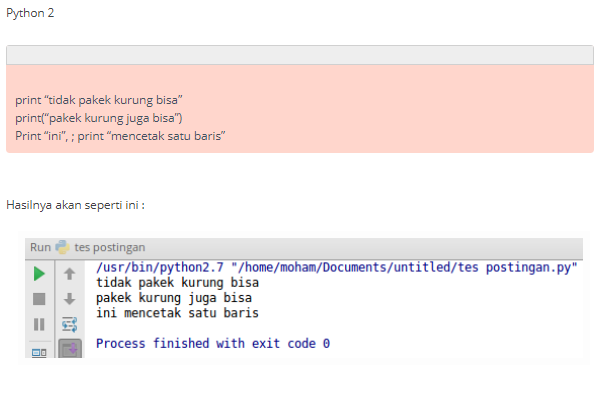
\includegraphics[width=15cm,height=16cm]{figures/1.PNG}
\caption{Python 2}
\label{penanda}
\end{figure}

\begin{figure}[!htbp]
\centering
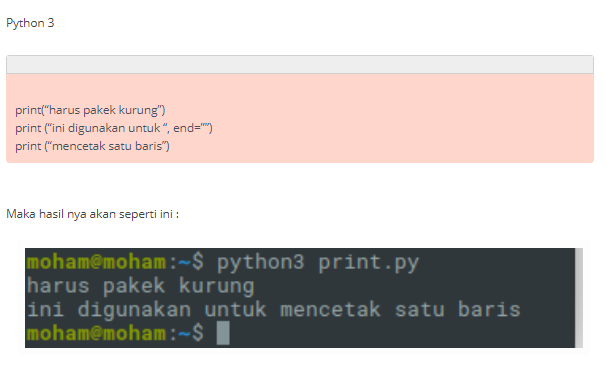
\includegraphics[width=15cm,height=16cm]{figures/2.PNG}
\caption{Python 3}
\label{penanda}
\end{figure}

\item 
Syntax untuk meminta inputan.
\\
\\
\\
\begin{figure}[!htbp]
\centering
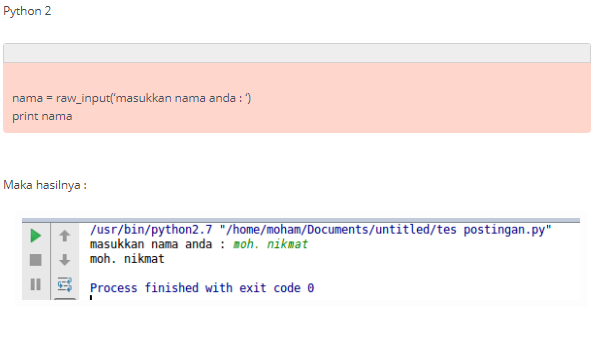
\includegraphics[width=15cm,height=18cm]{figures/3.PNG}
\caption{Python 2}
\label{penanda}
\end{figure}

\begin{figure}[!htbp]
\centering
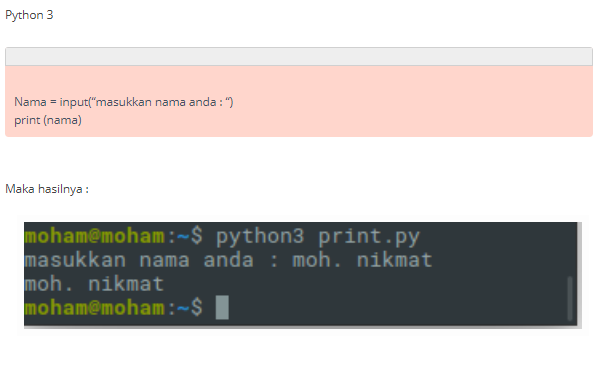
\includegraphics[width=15cm,height=15cm]{figures/4.PNG}
\caption{Python 3 dan hasil}
\label{penanda}
\end{figure}

\item 
Hasil dari operator pembagian.
\\
\\
\\
\begin{figure}[!htbp]
\centering
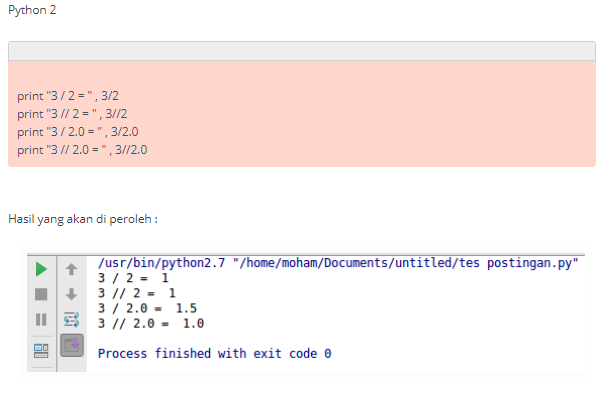
\includegraphics[width=15cm,height=15cm]{figures/5.PNG}
\caption{Python 2}
\label{penanda}
\end{figure}

\begin{figure}[!htbp]
\centering
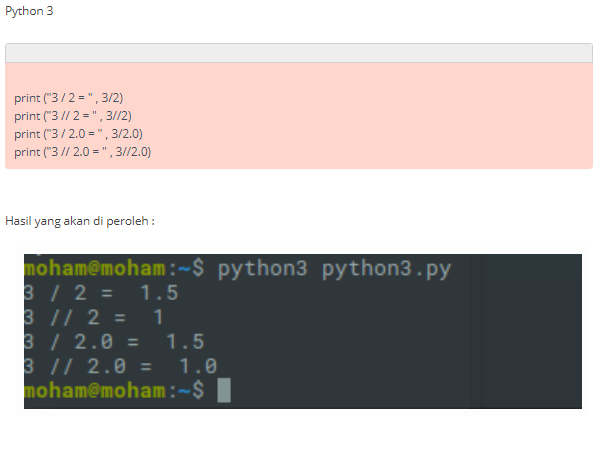
\includegraphics[width=15cm,height=15cm]{figures/6.PNG}
\caption{Python 3}
\label{penanda}
\end{figure}

\end{enumerate}
\section{Instalasi}
\subsection{Anaconda}
\par 
		Anaconda adalah perusahaan pengembang dan juga pengembang perangkat lunak pendukung sumber terbuka yang berbasis di Austin, Texas, AS. Berkomitmen untuk \textit{open source}, dan juga menciptakan distribusi dari Anaconda Python dan berkontribusi pada banyak alat analisis data berbasis sumber terbuka lainnya.

\subsubsection{Cara install Anaconda}
\par
	Sebelum \textit{menginstall} \textit{Anaconda Python} hal pertama yang harus diperhatikan yaitu versi dari Sistem Operasi yang digunakan, misalnya \textit{Windows} versi 32bit atau 64bit, jadi anda harus \textit{menginstall} \textit{Anaconda Python} sesuai dengan Sistem Operasi di \textit{windows} anda, karena jika versi \textit{windows} berbeda versi dengan \textit{Anaconda Python} dapat menyebabkan \textit{error}.\\
\begin{enumerate}
\item \textit{Download Anaconda Python} https://www.anaconda.com/distribution/

\item Buka aplikasi \textit{installer Anaconda} tersebut lalu akan muncul  gambar \textit{installer anaconda}.

\begin{figure}[!htbp]
    \centering
    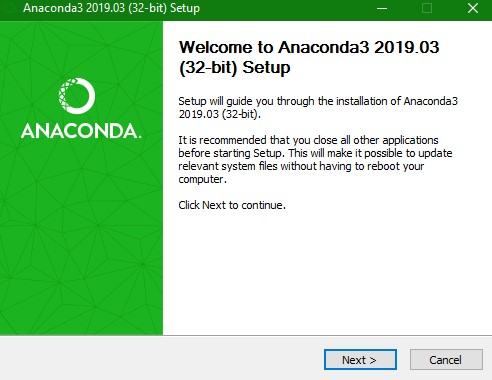
\includegraphics[scale=0.5]{figures/b.jpg}
    \caption{\textit{Installer anaconda}}
    \label{Figureanaconda2}
\end{figure}

\item Kemudian klik \textit{next}
\item Pada \textit{License Agreement} klik \textit{I Agree}
 gambar \textit{License Agreement}.

\begin{figure}[!htbp]
    \centering
    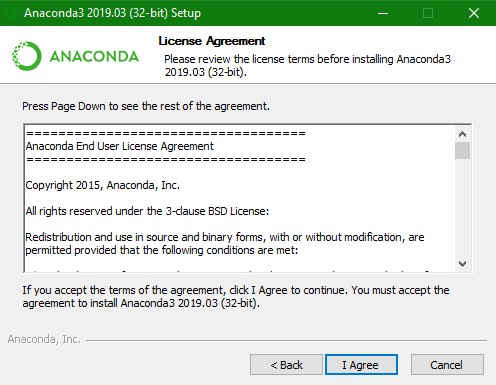
\includegraphics[scale=0.5]{figures/c.jpg}
    \caption{\textit{License Agreement}}
    \label{Figureanaconda3}
\end{figure}

\item Kemudian pilih \textit{Just Me(Recomended)} agar sesuai dengan komputer yang digunakan, kemudian klik \textit{next}
 gambar \textit{Just Me(recomended)}.

\begin{figure}[!htbp]
    \centering
    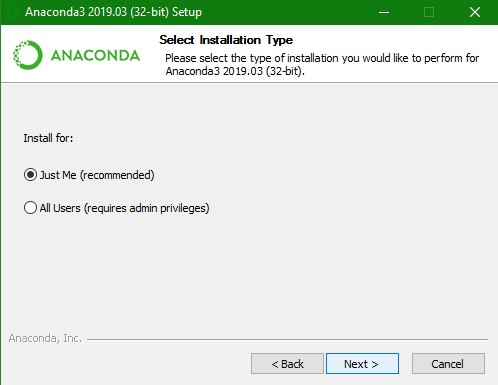
\includegraphics[scale=0.5]{figures/d.jpg}
    \caption{\textit{Just Me(recomended)}}
    \label{Figureanaconda4}
\end{figure}

\item Kemudian pilih lokasi tempat \textit{menginstall anaconda}
 gambar \textit{Pilih lokasi}.

\begin{figure}[!htbp]
    \centering
    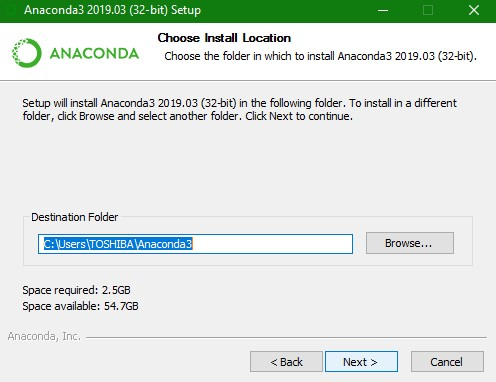
\includegraphics[scale=0.5]{figures/e.jpg}
    \caption{\textit{Pilih lokasi}}
    \label{Figureanaconda5}
\end{figure}

\item Kemudian centang \textit{Add Anaconda to my Path environtment variable}, agar saat \textit{menginstall selenium} langsung ke \textit{path anaconda} tidak ke aplikasi yang lain.
\item Klik \textit{install}
 gambar \textit{Centang Anaconda to my PATH}.

\begin{figure}[!htbp]
    \centering
    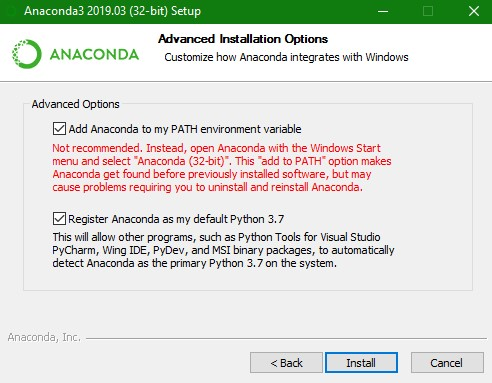
\includegraphics[scale=0.5]{figures/f.jpg}
    \caption{\textit{Centang Anaconda to my PATH}}
    \label{Figureanaconda6}
\end{figure}

\item Tunggu sampai proses \textit{installasi} selesai
 gambar \textit{Installation Complete}.

\begin{figure}[!htbp]
    \centering
    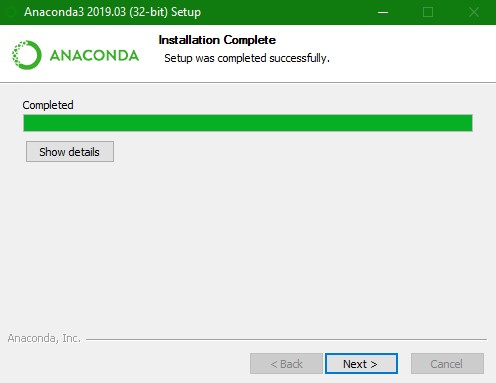
\includegraphics[scale=0.5]{figures/g.jpg}
    \caption{\textit{Installation Complete}}
    \label{Figureanaconda7}
\end{figure}

\item Klik \textit{next}

 gambar \textit{Anaconda+JetBrains}.

\begin{figure}[!htbp]
    \centering
    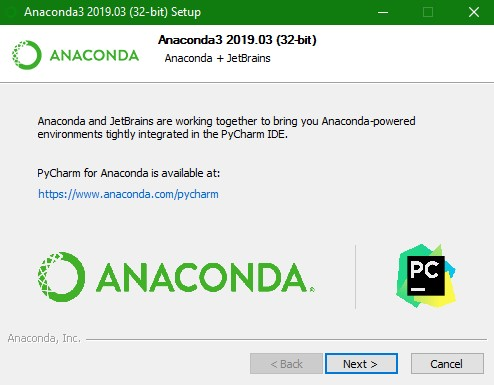
\includegraphics[scale=0.5]{figures/h.jpg}
    \caption{\textit{Anaconda+JetBrains}}
    \label{Figureanaconda8}
\end{figure}

\item klik \textit{next}
\item Jika sudah klik \textit{finish}

 gambar \textit{Thanks fo install Anaconda}.

\begin{figure}[!htbp]
    \centering
    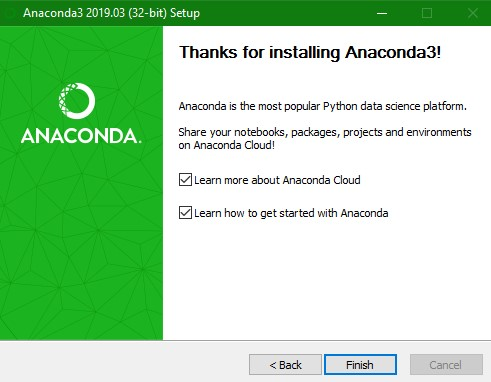
\includegraphics[scale=0.5]{figures/qz.jpg}
    \caption{\textit{Thanks for install Anaconda}}
    \label{Figureanaconda70}
\end{figure}
\\
\end{enumerate}
\\
\subsection{Python}
\par
    Python merupakan bahasa pemrograman yang interpreatatif multiguna dengan suatu filosofi perancangan yang sangat berfokus pada tingkat keterbacaan kode. Python disebut juga sebagai bahasa yang kemampuan yait muenggabungkan kapabilitas, dan sintaksis kode yang sangat terperinci, dan juga dilengkapi dengan berbagai fungsionalitas pustaka terstandar yang luas dan besar serta komprehensif.
\subsubsection{Cara Menginstall Python}
\par
\begin{enumerate}
    \item \textit{Download Python}
    https://www.python.org/downloads/windows/.
    \item Buka aplikasi \textit{installer Python} tersebut lalu akan muncul  gambar \textit{installer Now}.
    \begin{figure}[!htbp]
    \centering
    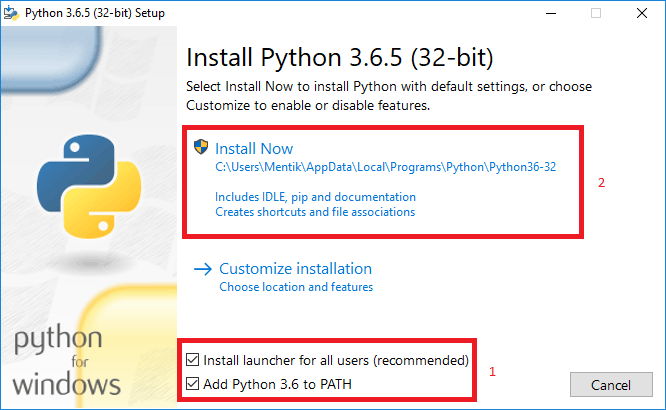
\includegraphics[scale=0.5]{figures/i.png}
    \caption{\textit{Installer Python}}
    \label{Figurepython}
    \end{figure}
\item Proses Installer.
     \begin{figure}[!htbp]
    \centering
    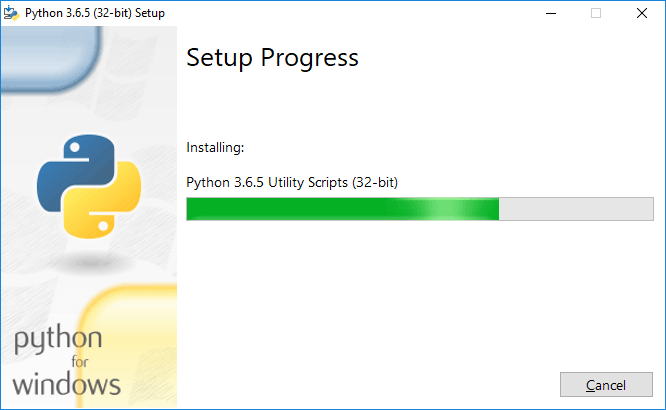
\includegraphics[scale=0.5]{figures/g.png}
    \caption{\textit{Installer Python}}
    \label{Figurepython}
    \end{figure}
\item Tunggu sampai proses \textit{installasi} selesai
 gambar \textit{Installation Complete}.
    \begin{figure}[!htbp]
    \centering
    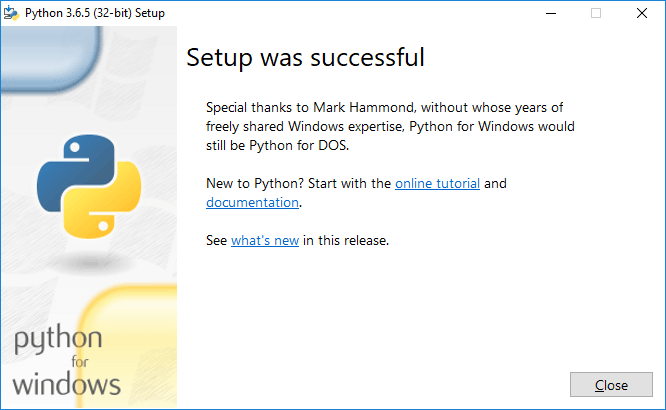
\includegraphics[scale=0.5]{figures/j.png}
    \caption{\textit{Installer Python}}
    \label{Figurepython}
    \end{figure}
\end{enumerate}
\subsection{PIP Python}
\subsubsection{Cara Menginstall PIP-Python}
\begin{enumerate}
\item \textit{Download Pip.py}
    di link https://pip.pypa.io/en/stable/installing/
    \begin{figure}[!htbp]
    \centering
    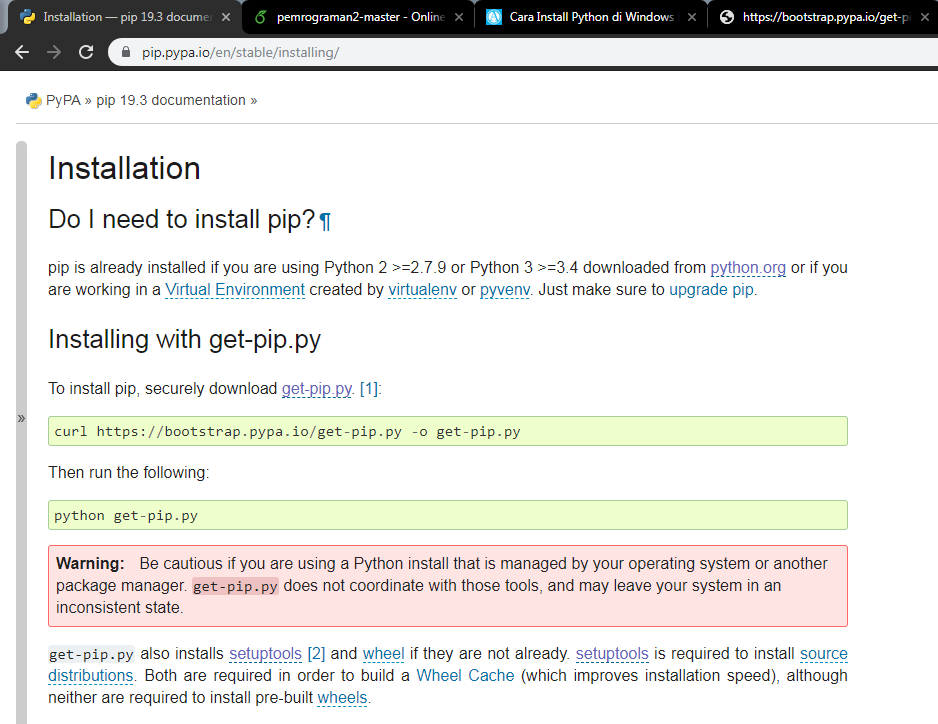
\includegraphics[scale=0.5]{figures/pip11.PNG}
    \caption{\textit{Installer Pip}}
    \label{Figurepython}
    \end{figure}
\item Klik Kanan lalu Save file .py
     \begin{figure}[!htbp]
    \centering
    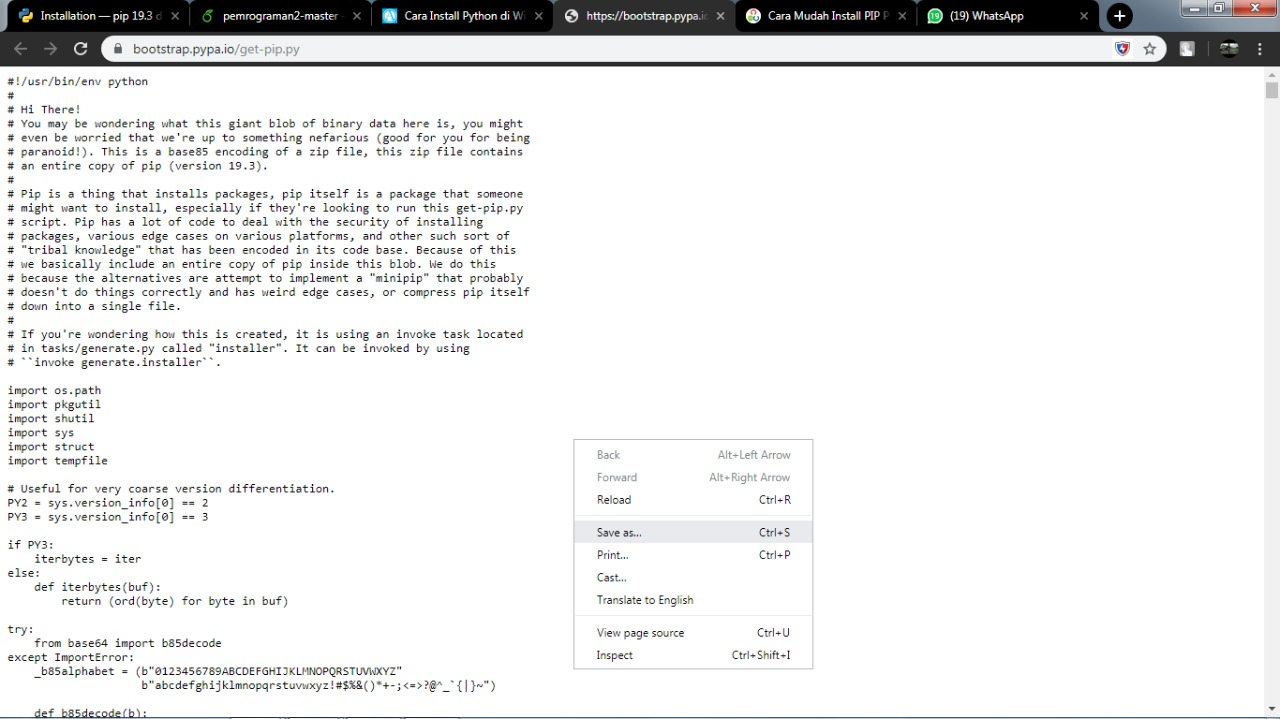
\includegraphics[scale=0.2]{figures/pip12.png}
    \caption{\textit{Installer Pip}}
    \label{Figurepython}
    \end{figure}
 \item lalu klik file, tunggu hingga selesai.
 \item kemudian buka cmd (Command Prompt) ketik \textit{Pip -v}
     \begin{figure}[!htbp]
    \centering
    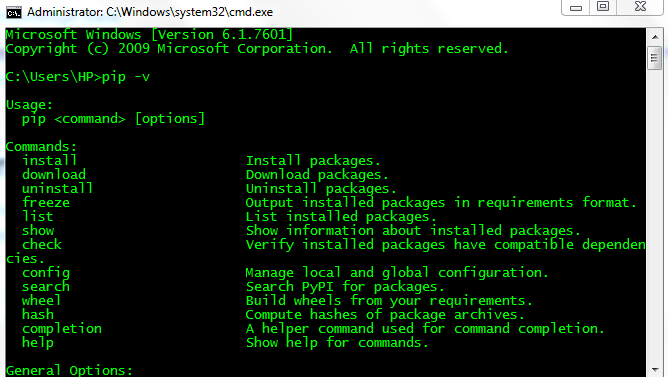
\includegraphics[scale=0.5]{figures/pip1.PNG}
    \caption{\textit{Installer Pip}}
    \label{Figurepython}
    \end{figure}
\item lalu ketik \textit{Python -m pip install --upgrade pip}
     \begin{figure}[!htbp]
    \centering
    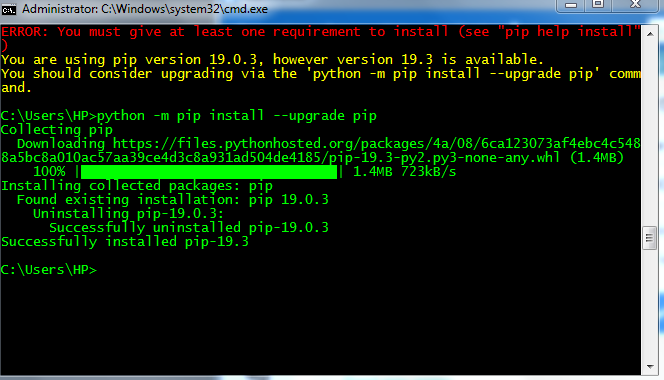
\includegraphics[scale=0.5]{figures/pip2.PNG}
    \caption{\textit{Installer Pip}}
    \label{Figurepython}
    \end{figure}
 \item Install Pip selesai.
 \end{enumerate}
\subsection{Cara Setting Environment}
\begin{enumerate}
\item Pergi Ke Run Pada Menu Start, ketik\textit{sysdm.cpl}
\item Kemudian Akan Ditampilkan seprti dibawah, Pilih Advance. 
    \begin{figure}[!htbp]
    \centering
    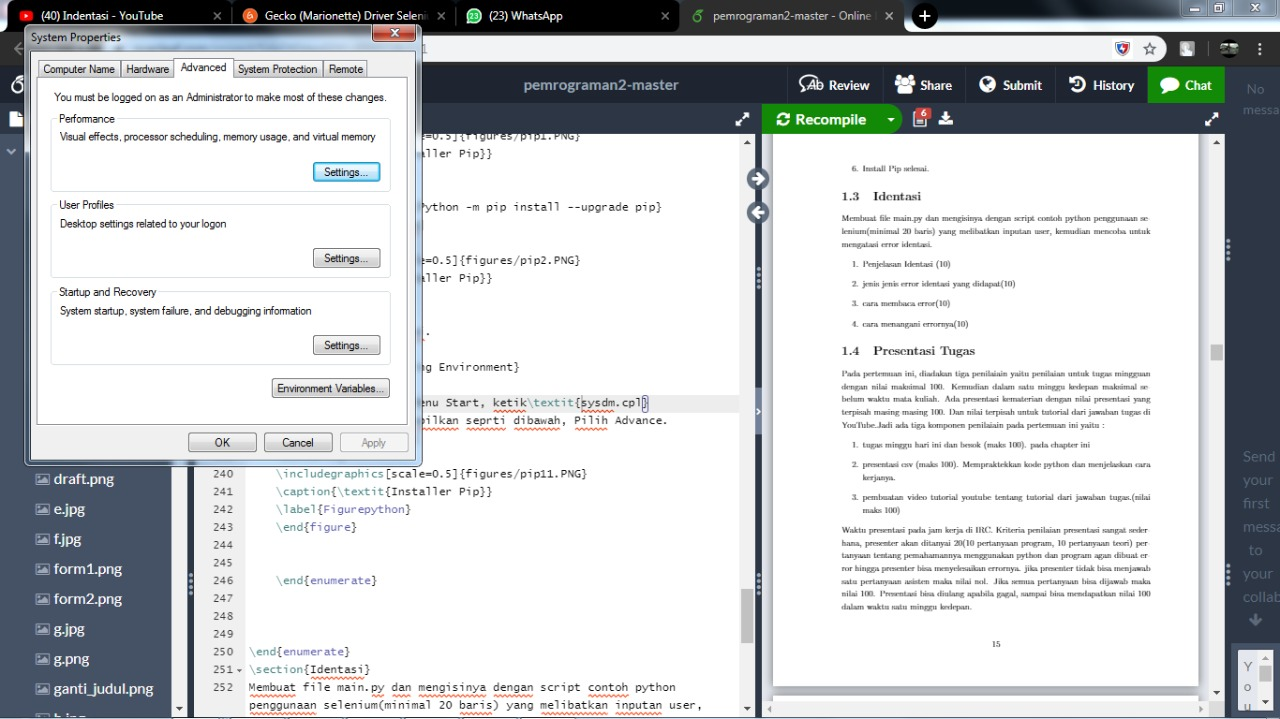
\includegraphics[scale=0.2]{figures/21.PNG}
    \caption{\textit{Setting Environment}}
    \label{Figurepython}
    \end{figure}
\item Klik Environment Variables, Cari Path lalu edit.
\begin{figure}[!htbp]
    \centering
    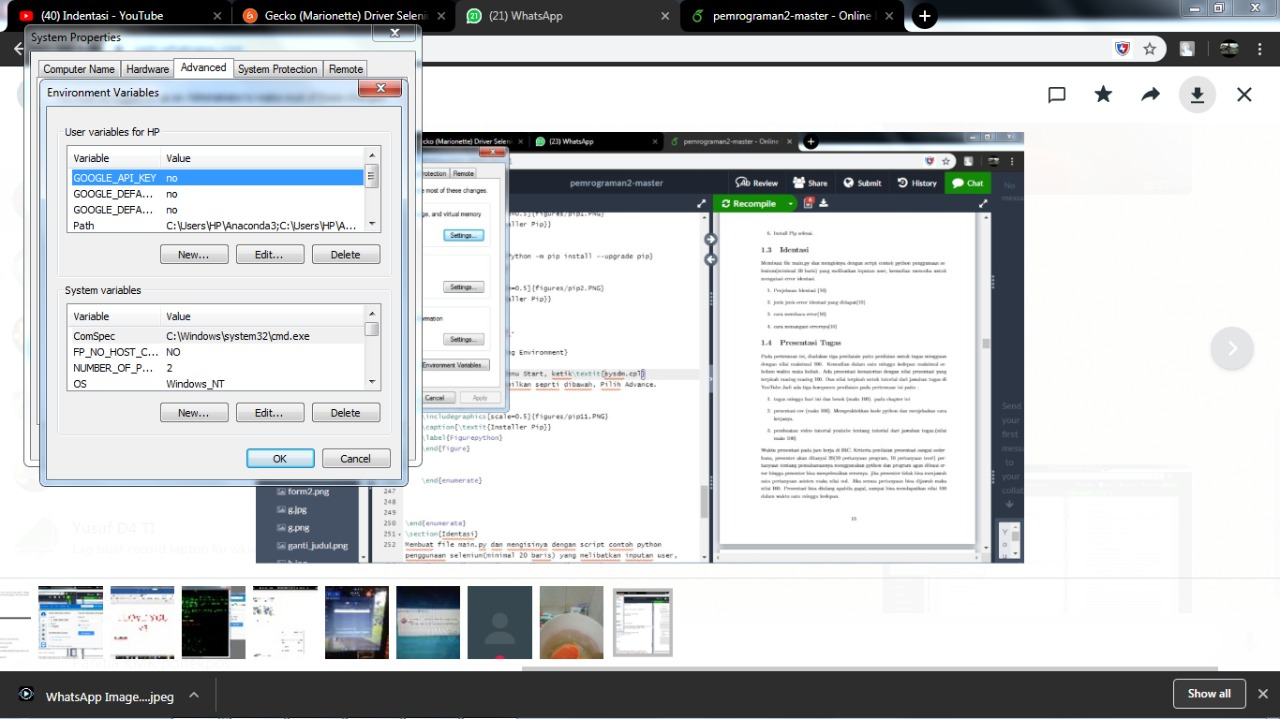
\includegraphics[scale=0.3]{figures/22.PNG}
    \caption{\textit{Setting Environment}}
    \label{Figurepython}
    \end{figure}
\item Edit menjadi \textit{C:System35/Scripts}, lalu tekan OKE
\begin{figure}[!htbp]
    \centering
    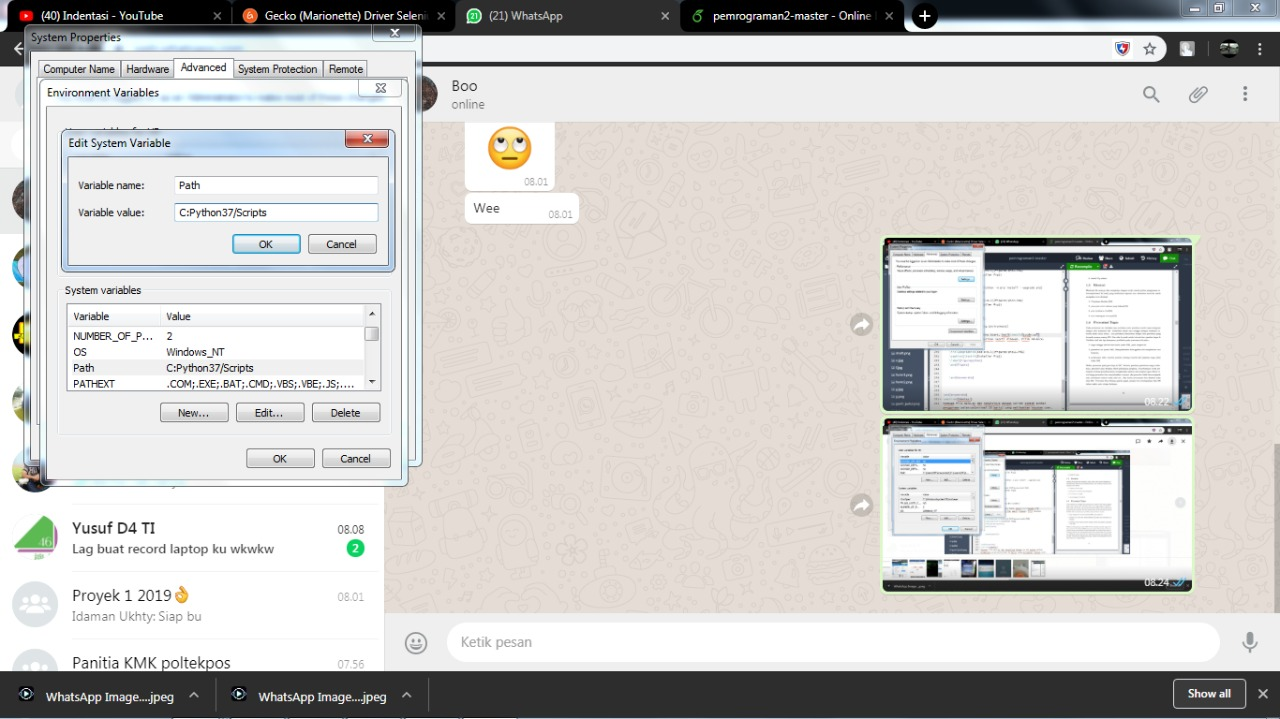
\includegraphics[scale=0.2]{figures/23.PNG}
    \caption{\textit{Installer Pip}}
    \label{Figurepython}
    \end{figure}
    
\item Selesai
\end{enumerate}

\subsection{Mencoba entrepreter/cli melalui terminal atau cmd windows}
\begin{enumerate}
    \item Klik tombol Start, Kemudian Ketik \textit{cmd}
    \item Ketik\textit{Python}
\item kemudian ketik \textit{Print("hello world")}     
    \begin{figure}[!htbp]
    \centering
    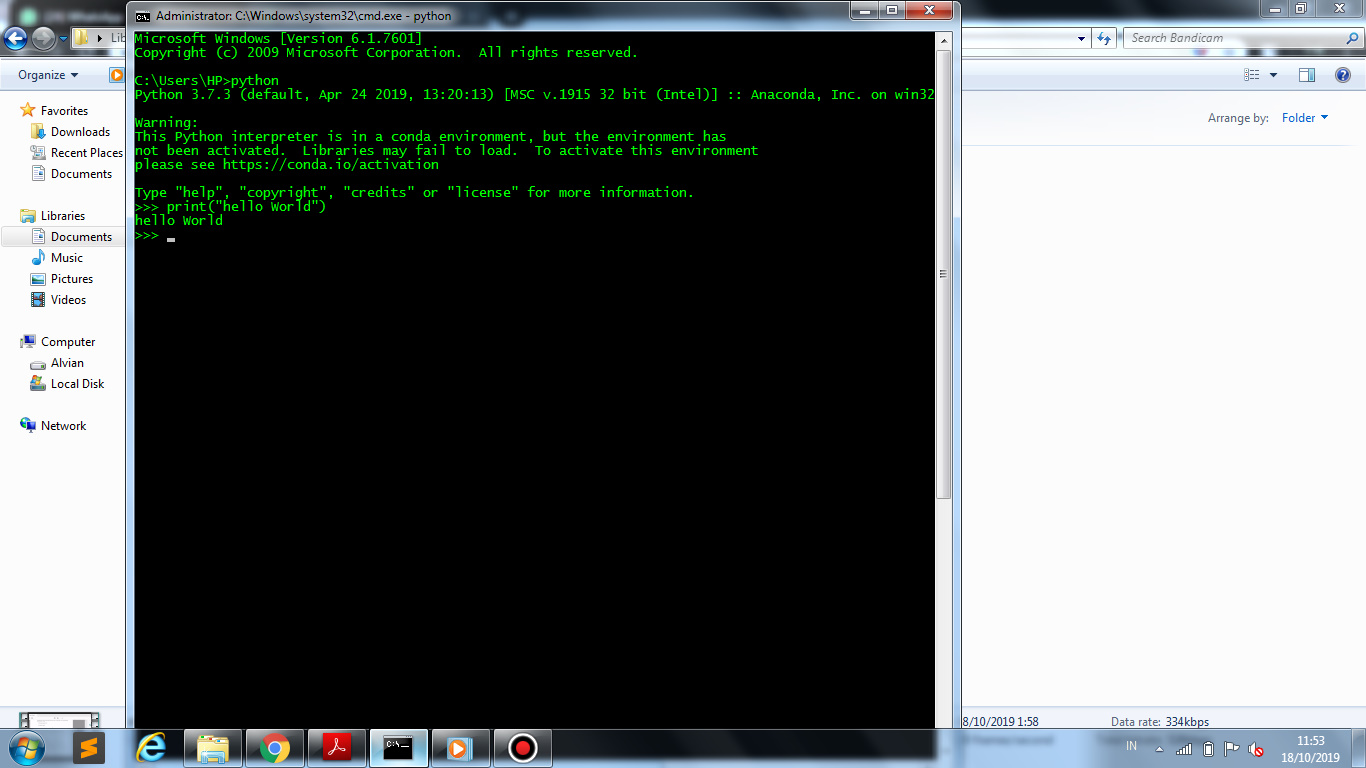
\includegraphics[scale=0.2]{figures/24.PNG}
    \caption{\textit{Mencoba entrepreter/cli melalui terminal atau cmd windows}}
    \label{Figurepython}
    \end{figure}
\item Kemudian selesai.     
\end{enumerate}
\subsection{Menjalankan dan mengupdate anaconda dan spyder}
\begin{enumerate}
    \item Buka cmd pada tombol Start.
    \item Kemudian klik \textit{conda install -c anaconda python}
    \begin{figure}[!htbp]
    \centering
    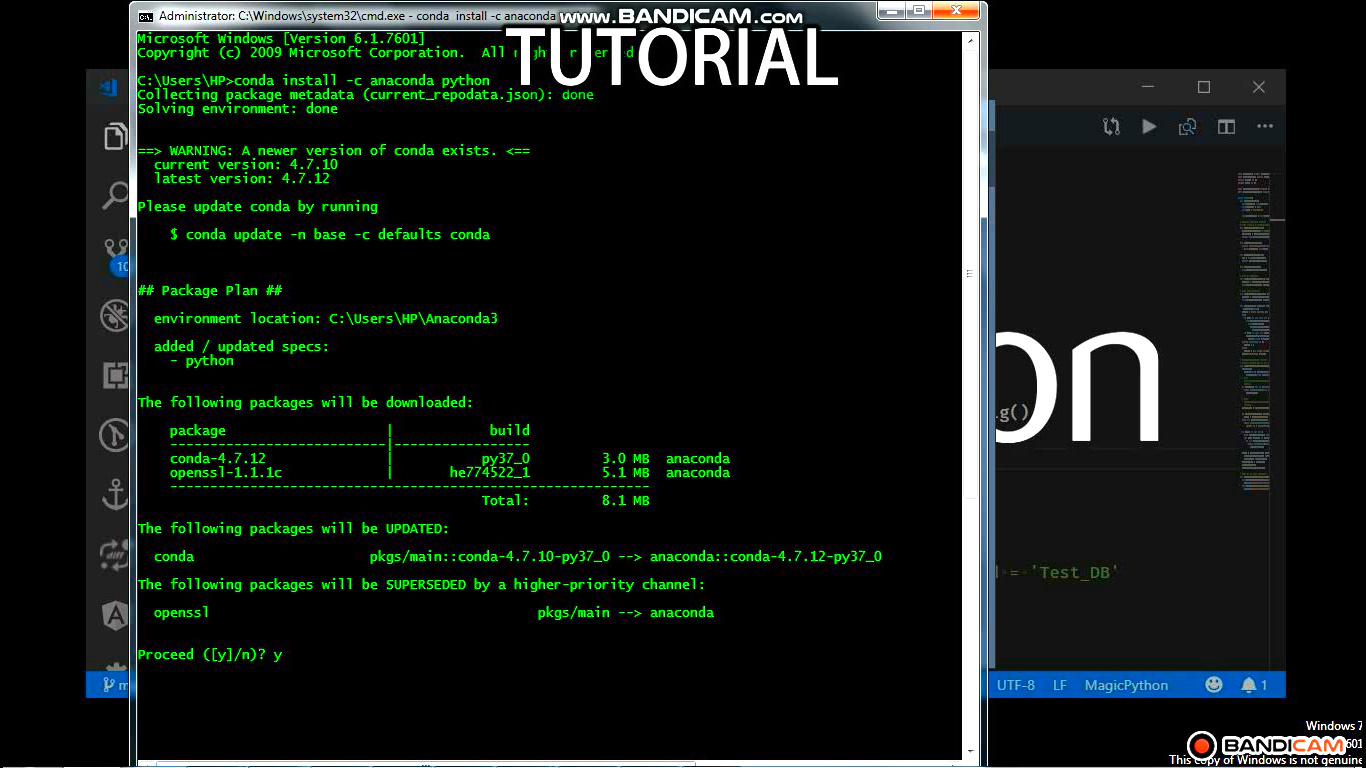
\includegraphics[scale=0.2]{figures/25.PNG}
    \caption{\textit{Menjalankan dan mengupdate anaconda dan spyder}}
    \label{Figurepython}
    \end{figure}
\end{enumerate}
\subsection{Cara menjalankan Script hello word di Spyder}
\begin{enumerate}
    \item Pertama, Pastikan anda sudah berada di aplikasi Spyder.
    \item Kemudian Ketik \textit{
    Alvian = ('Hello world')
    print("Hello World") }
\item maka Akan ditampilkan sebagai berikut.
    \begin{figure}[!htbp]
    \centering
    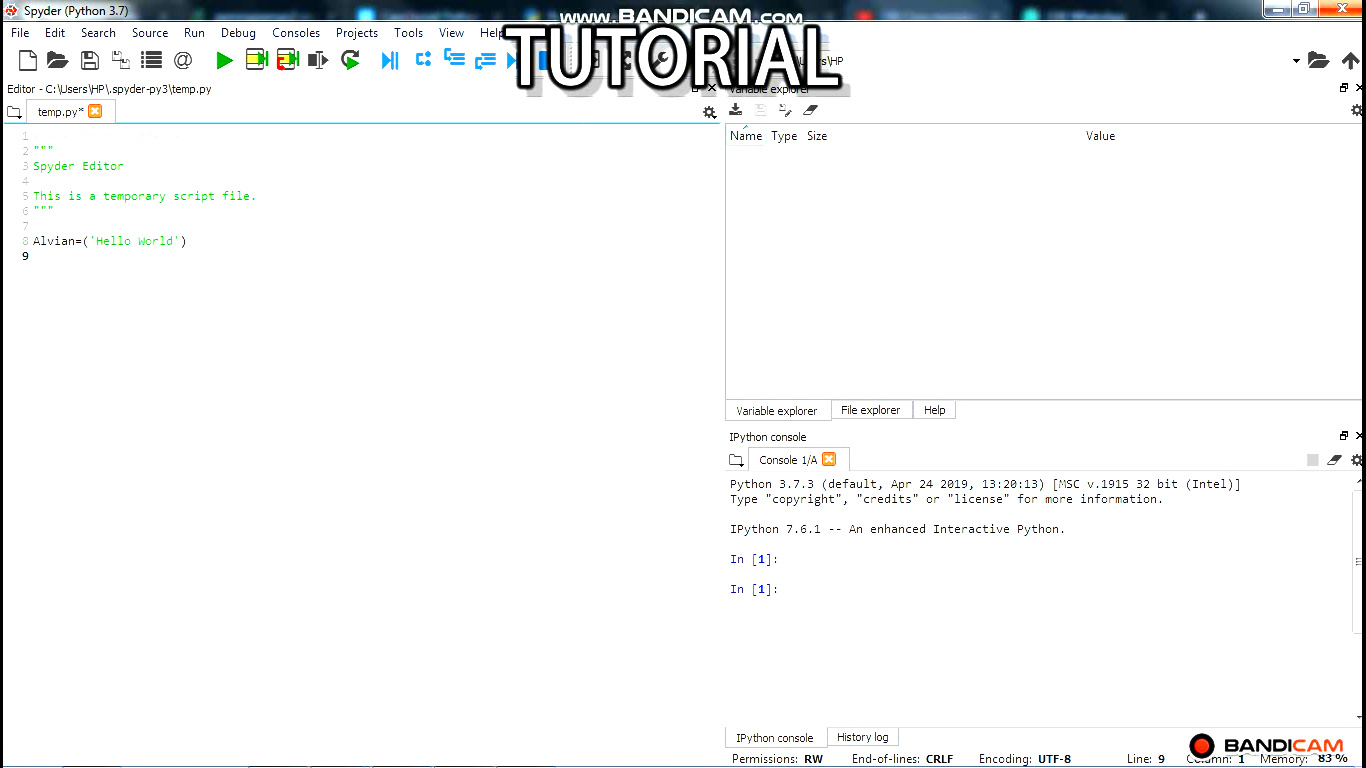
\includegraphics[scale=0.2]{figures/26.PNG}
    \caption{\textit{Cara menjalankan Script hello word di Spyder}}
    \label{Figurepython}
    \end{figure}
\end{enumerate}
\subsection{Cara pemakaian variable explorer di Spyder}
\begin{enumerate}

    \item Pertama, Pastikan anda sudah berada di aplikasi Spyder.
    \item Kemudian Ketik \textit{
    Alvian = ('Hello world')
    print("Hello World")}
\item kemudian tekan variabel explorer.
    \begin{figure}[!htbp]
    \centering
    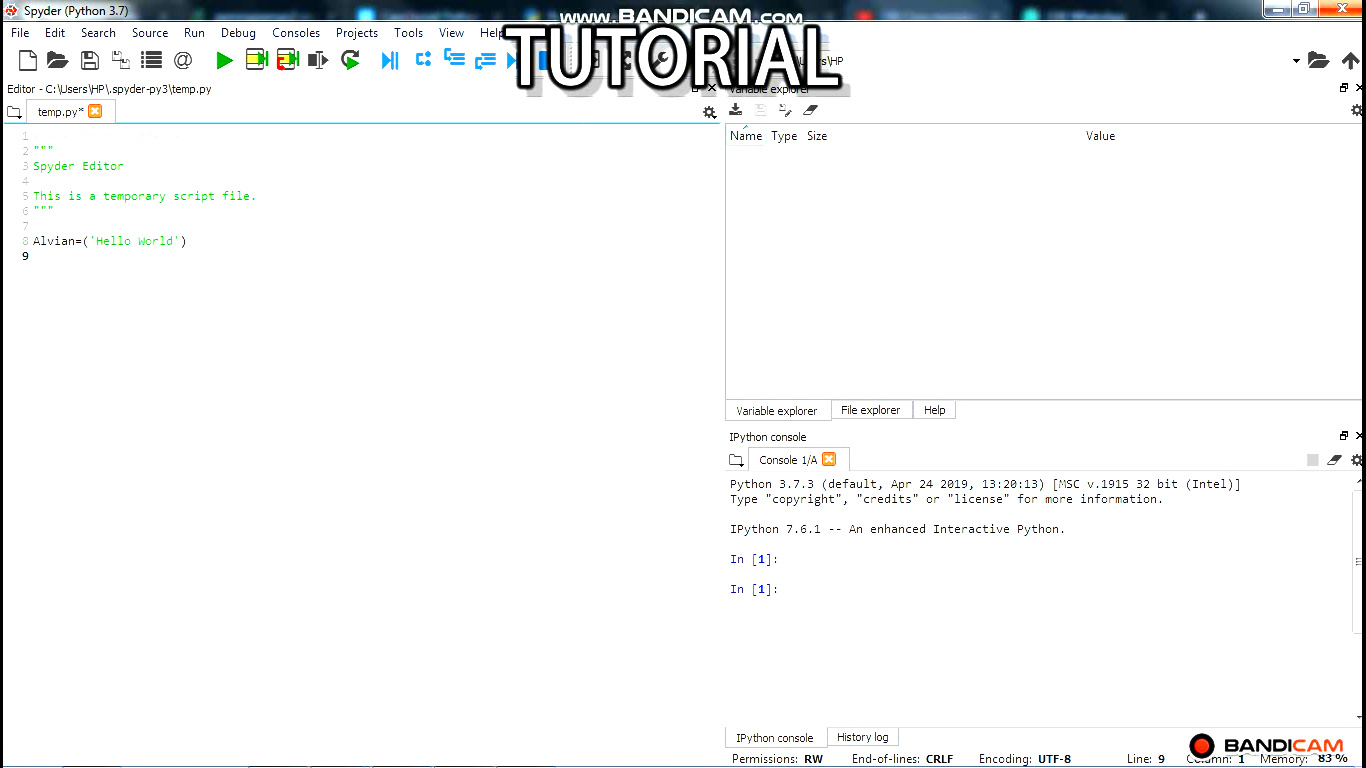
\includegraphics[scale=0.2]{figures/26.PNG}
    \caption{\textit{Cara pemakaian variable explorer di Spyder}}
    \label{Figurepython}
    \end{figure}
\end{enumerate}
\subsection{Cara menjalankan Script otomatis login aplikasi akademik dengan library sele-
nium dan inputan user}
\begin{enumerate}
    \item Pertama Masuk pada \textit{Spyder}
    \item ketik Pada Spyder \textit{ from selenium.webdriver import Firefox
    from selenium.webdriver.firefox.options import Options
    from selenium.webdriver.common.desired_capabilities import DesiredCapabilities
    from selenium.webdriver.firefox.firefox_binary import FirefoxBinary
    opsi = Options()
    opsi.headless = False
    binary = FirefoxBinary("C:\\Program Files\\Mozilla Firefox\\firefox.exe")
    cap = DesiredCapabilities().FIREFOX
    cap['marionette'] = True
    browser=Firefox(executable_path='geckodriver.exe',options=opsi,capabilities=cap,firefox_binary=binary)
    browser.get('http://siap.poltekpos.ac.id/siap/besan.depan.php')
    browser.find_element_by_name('user_name').send_keys("masukin npm")
    browser.find_element_by_name('user_pass').send_keys("masukin pass")
    browser.find_element_by_xpath('/html/body/table/tbody/tr[5]/td/table[1]/tbody/tr/td[2]/table[2]/tbody/tr[1]/td[2]/div/form/input[4]').click()}
    \item pastikan anda Sudah menginstal Geckodriver.exe
    \begin{figure}[!htbp]
    \centering
    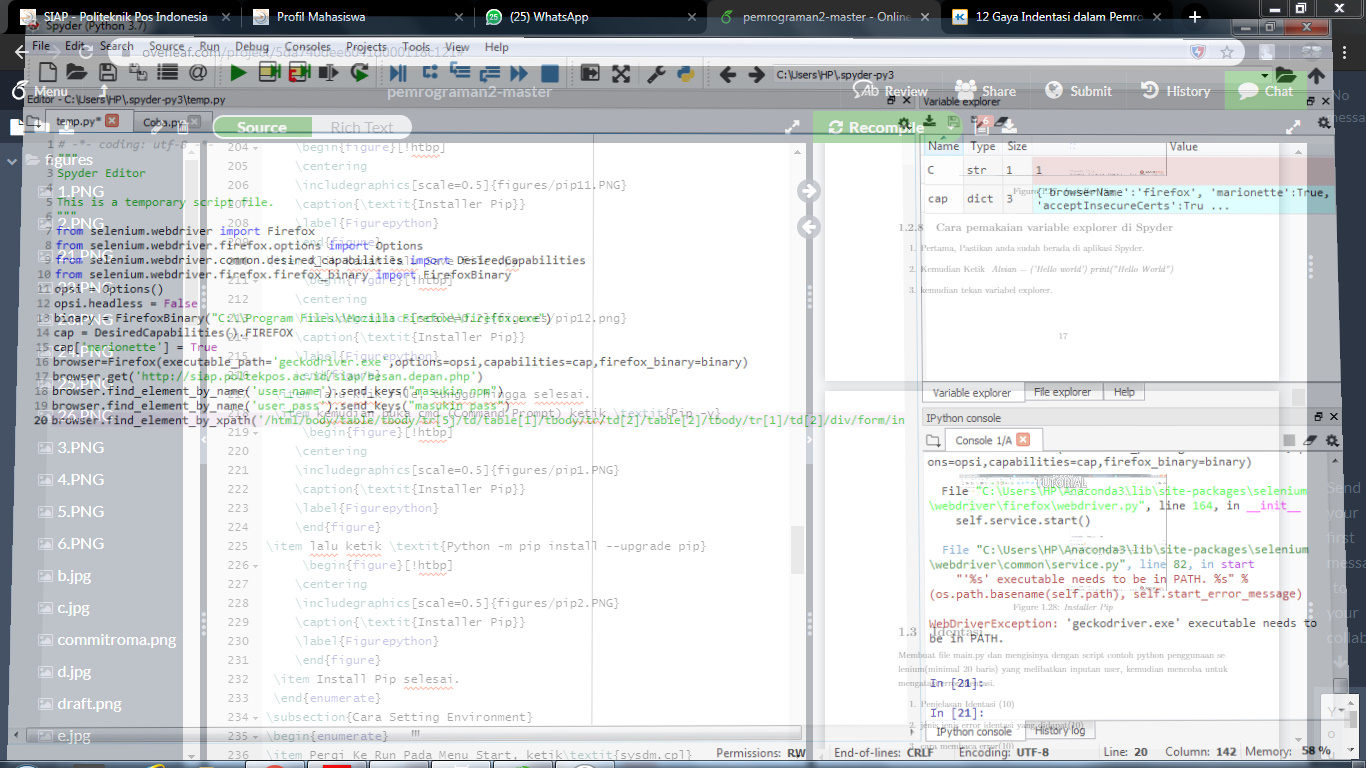
\includegraphics[scale=0.2]{figures/27.jpg}
    \caption{\textit{Menjalankan Scripts Otomatis}}
    \label{Figurepython}
    \end{figure}
    \item dan akan otomatis langsung masuk pada alamat url yang dimasukkan dan login otomatis.
\end{enumerate}

\section{Indentasi}
\begin{enumerate}
	\item Indentasi adalah salah satu langkah atau cara untuk merapikan sintaks dalam pemrograman yang hendak ditulis atau dibuat. Dan indentasi, ternyata digunakan sebagai salah satu acuan scope pemrograman dan compiler seperti bahasa pemrograman Python. Indentasi selalu berhubungan dengan kurung kurawal '{}' dalam mengakhiri dan mememulai suatu scope pemrograman.
	\item Spasi Pada \textit{Print (x)}
	\begin{figure}[!htbp]
    \centering
    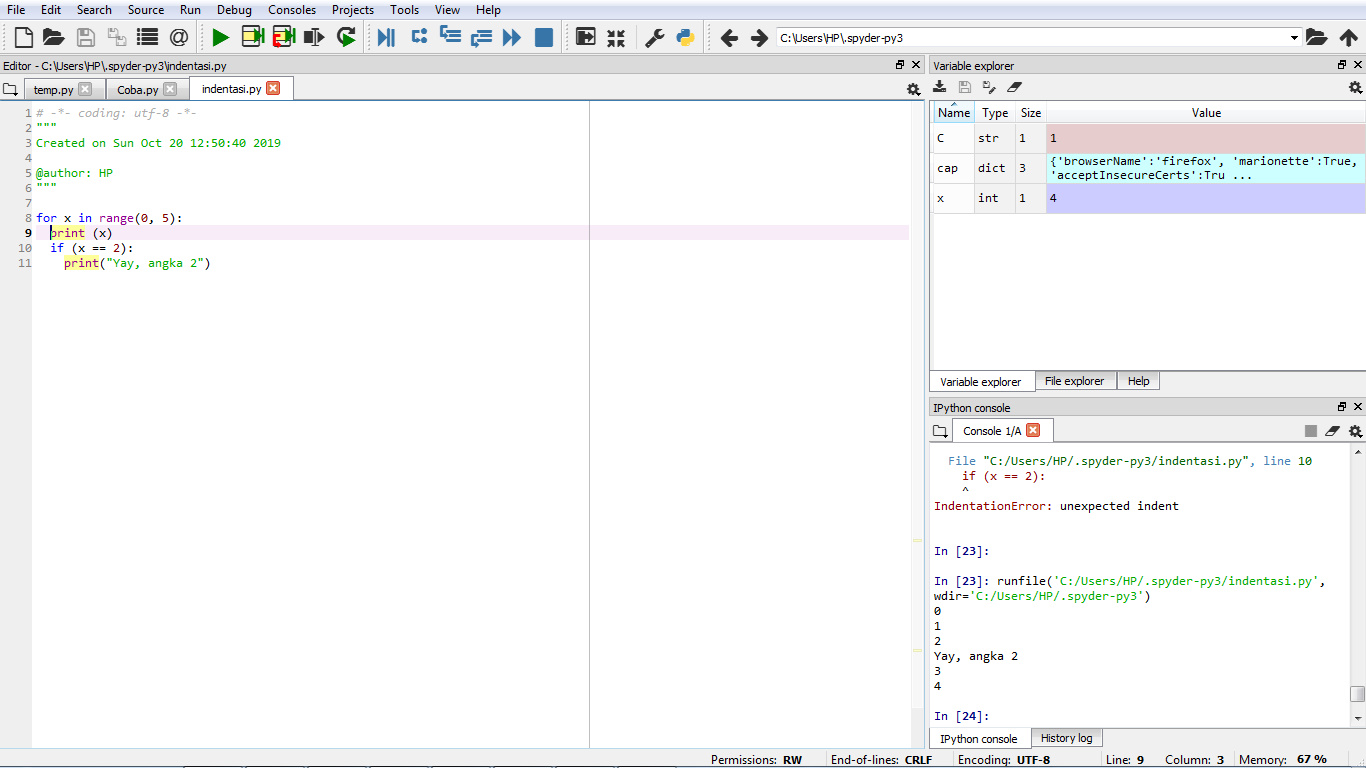
\includegraphics[scale=0.2]{figures/30.PNG}
    \caption{\textit{Indentasi}}
    \label{Figurepython}
    \end{figure}
\item Cara membaca eror
\par
Pertama Liat apa yang eror pada Console , kemudia terjemahkan kalimata pada cosole cari masalah , biasaya jika masalahnya da pada indetasinya , maka konsol akan mengeluarkan kata yaitu \textit{IndentationError: expected an indented block}
	\begin{figure}[!htbp]
    \centering
    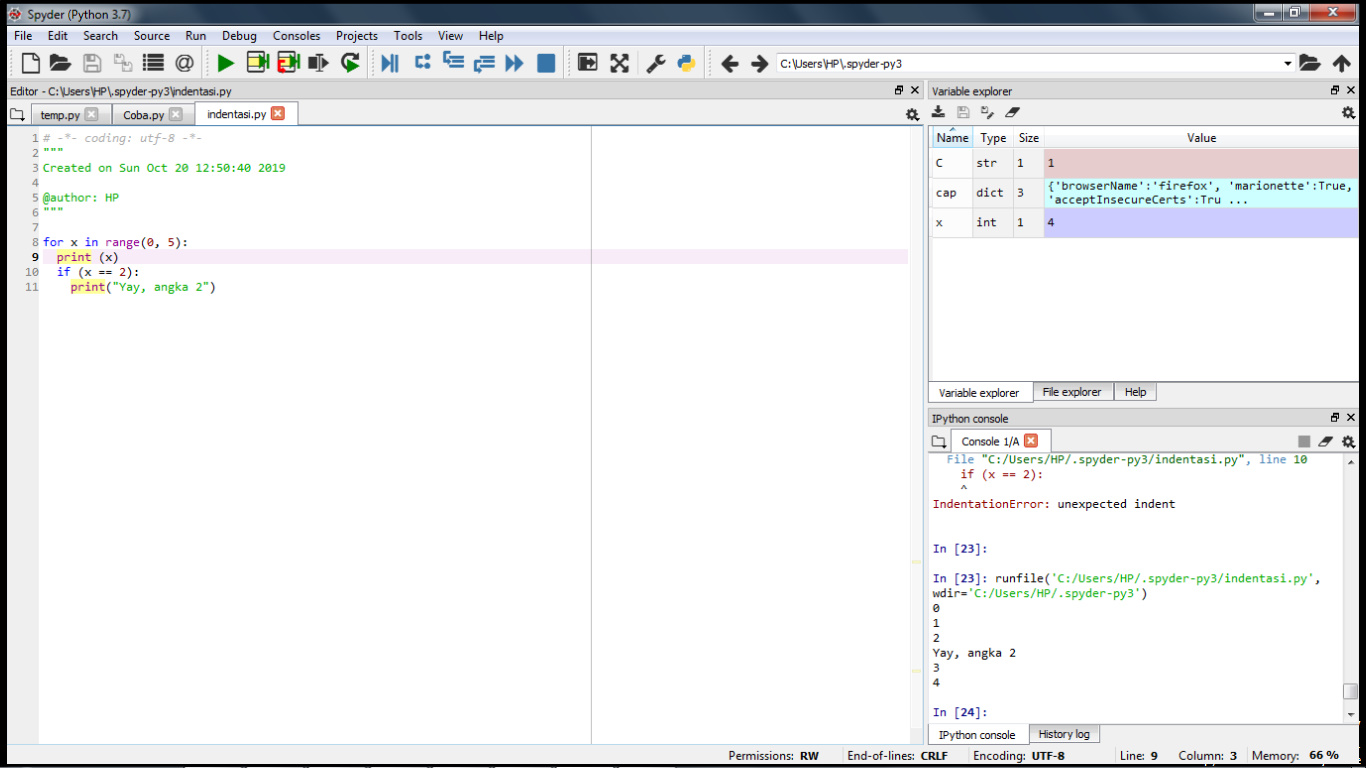
\includegraphics[scale=0.2]{figures/31.PNG}
    \caption{\textit{Indentasi}}
    \label{Figurepython}
    \end{figure}
\item cara menangani errornya.
\par
Cara menanggapin eror adalah dengan bersyukur.
\end{enumerate}
